%% BioMed_Central_Tex_Template_v1.06
%%                                      %
%  bmc_article.tex            ver: 1.06 %
%                                       %

%%IMPORTANT: do not delete the first line of this template
%%It must be present to enable the BMC Submission system to
%%recognise this template!!

%%%%%%%%%%%%%%%%%%%%%%%%%%%%%%%%%%%%%%%%%
%%                                     %%
%%  LaTeX template for BioMed Central  %%
%%     journal article submissions     %%
%%                                     %%
%%          <8 June 2012>              %%
%%                                     %%
%%                                     %%
%%%%%%%%%%%%%%%%%%%%%%%%%%%%%%%%%%%%%%%%%


%%%%%%%%%%%%%%%%%%%%%%%%%%%%%%%%%%%%%%%%%%%%%%%%%%%%%%%%%%%%%%%%%%%%%
%%                                                                 %%
%% For instructions on how to fill out this Tex template           %%
%% document please refer to Readme.html and the instructions for   %%
%% authors page on the biomed central website                      %%
%% http://www.biomedcentral.com/info/authors/                      %%
%%                                                                 %%
%% Please do not use \input{...} to include other tex files.       %%
%% Submit your LaTeX manuscript as one .tex document.              %%
%%                                                                 %%
%% All additional figures and files should be attached             %%
%% separately and not embedded in the \TeX\ document itself.       %%
%%                                                                 %%
%% BioMed Central currently use the MikTex distribution of         %%
%% TeX for Windows) of TeX and LaTeX.  This is available from      %%
%% http://www.miktex.org                                           %%
%%                                                                 %%
%%%%%%%%%%%%%%%%%%%%%%%%%%%%%%%%%%%%%%%%%%%%%%%%%%%%%%%%%%%%%%%%%%%%%

%%% additional documentclass options:
%  [doublespacing]
%  [linenumbers]   - put the line numbers on margins

%%% loading packages, author definitions

%\documentclass[twocolumn]{bmcart}% uncomment this for twocolumn layout and comment line below
\documentclass{bmcart}

%%% Load packages
\usepackage{amsthm,amsmath}
\RequirePackage[square,numbers,sort&compress]{natbib}
%\RequirePackage[authoryear]{natbib}% uncomment this for author-year bibliography
\usepackage[pdftex]{graphicx}
\usepackage{hyperref}
\usepackage[utf8]{inputenc} %unicode support
%\usepackage[applemac]{inputenc} %applemac support if unicode package fails
%\usepackage[latin1]{inputenc} %UNIX support if unicode package fails
\usepackage{url}
\usepackage{lmodern}

%%%%%%%%%%%%%%%%%%%%%%%%%%%%%%%%%%%%%%%%%%%%%%%%%
%%                                             %%
%%  If you wish to display your graphics for   %%
%%  your own use using includegraphic or       %%
%%  includegraphics, then comment out the      %%
%%  following two lines of code.               %%
%%  NB: These line *must* be included when     %%
%%  submitting to BMC.                         %%
%%  All figure files must be submitted as      %%
%%  separate graphics through the BMC          %%
%%  submission process, not included in the    %%
%%  submitted article.                         %%
%%                                             %%
%%%%%%%%%%%%%%%%%%%%%%%%%%%%%%%%%%%%%%%%%%%%%%%%%


%\def\includegraphic{}
%\def\includegraphics{}

%%% Put your definitions there:
\startlocaldefs
\newcommand{\sbmlpkg}{SBMLPkgSpec}
\newcommand{\sbmlpkgfile}{\texttt{sbmlpkgspec.cls}}
\newcommand{\githuburl}{https://github.com/sbmlteam/sbmlpkgspec}
\endlocaldefs


%%% Begin ...
\begin{document}

%%% Start of article front matter
\begin{frontmatter}

\begin{fmbox}
\dochead{Research}

%%%%%%%%%%%%%%%%%%%%%%%%%%%%%%%%%%%%%%%%%%%%%%
%%                                          %%
%% Enter the title of your article here     %%
%%                                          %%
%%%%%%%%%%%%%%%%%%%%%%%%%%%%%%%%%%%%%%%%%%%%%%

\title{\sbmlpkg: A LaTeX Style File for SBML Package Specification Documents}

%%%%%%%%%%%%%%%%%%%%%%%%%%%%%%%%%%%%%%%%%%%%%%
%%                                          %%
%% Enter the authors here                   %%
%%                                          %%
%% Specify information, if available,       %%
%% in the form:                             %%
%%   <key>={<id1>,<id2>}                    %%
%%   <key>=                                 %%
%% Comment or delete the keys which are     %%
%% not used. Repeat \author command as much %%
%% as required.                             %%
%%                                          %%
%%%%%%%%%%%%%%%%%%%%%%%%%%%%%%%%%%%%%%%%%%%%%%

\author[
   addressref={aff1},                   % id's of addresses, e.g. {aff1,aff2}
   corref={aff1},                       % id of corresponding address, if any
   %noteref={n1},                        % id's of article notes, if any
   email={mhucka@caltech.edu}   % email address
]{\inits{MH}\fnm{Michael} \snm{Hucka}}

%%%%%%%%%%%%%%%%%%%%%%%%%%%%%%%%%%%%%%%%%%%%%%
%%                                          %%
%% Enter the authors' addresses here        %%
%%                                          %%
%% Repeat \address commands as much as      %%
%% required.                                %%
%%                                          %%
%%%%%%%%%%%%%%%%%%%%%%%%%%%%%%%%%%%%%%%%%%%%%%

\address[id=aff1]{%                           % unique id
  \orgname{Department of Computing and Mathematical Sciences, California Institute of Technology}, % university, etc
  \street{1200 E. California Blvd.},
  %\postcode{91125}
  \city{Pasadena, California 91125},
  \cny{USA}
}

%%%%%%%%%%%%%%%%%%%%%%%%%%%%%%%%%%%%%%%%%%%%%%
%%                                          %%
%% Enter short notes here                   %%
%%                                          %%
%% Short notes will be after addresses      %%
%% on first page.                           %%
%%                                          %%
%%%%%%%%%%%%%%%%%%%%%%%%%%%%%%%%%%%%%%%%%%%%%%

\begin{artnotes}
%\note{Sample of title note}     % note to the article
%\note[id=n1]{Equal contributor} % note, connected to author
\end{artnotes}

\end{fmbox}% comment this for two column layout

%%%%%%%%%%%%%%%%%%%%%%%%%%%%%%%%%%%%%%%%%%%%%%
%%                                          %%
%% The Abstract begins here                 %%
%%                                          %%
%% Please refer to the Instructions for     %%
%% authors on http://www.biomedcentral.com  %%
%% and include the section headings         %%
%% accordingly for your article type.       %%
%%                                          %%
%%%%%%%%%%%%%%%%%%%%%%%%%%%%%%%%%%%%%%%%%%%%%%

\begin{abstractbox}

\begin{abstract}
\parttitle{Objective} SBML (the Systems Biology Markup Language) is a popular open format for storing and exchanging computational models in biology.  The definition of SBML is captured in formal specification documents.  \sbmlpkg{} is a LaTeX document style intended to fill the need for a standard format for writing such specification documents.

\parttitle{Results} Specification documents for SBML Level~3 extensions (known as \emph{packages} in SBML) are made more uniform with the use of a standard template.  \sbmlpkg{} is a LaTeX class that provides a document framework for SBML Level~3 package specifications, to simplify the work of document authors while improving the overall quality of the family of SBML specifications.
\end{abstract}

%%%%%%%%%%%%%%%%%%%%%%%%%%%%%%%%%%%%%%%%%%%%%%
%%                                          %%
%% The keywords begin here                  %%
%%                                          %%
%% Put each keyword in separate \kwd{}.     %%
%%                                          %%
%%%%%%%%%%%%%%%%%%%%%%%%%%%%%%%%%%%%%%%%%%%%%%

\begin{keyword}
\kwd{SBML}
\kwd{XML}
\kwd{data formats}
\kwd{software}
\kwd{simulation}
\kwd{systems biology}
\kwd{computational biology}
\end{keyword}

% MSC classifications codes, if any
%\begin{keyword}[class=AMS]
%\kwd[Primary ]{}
%\kwd{}
%\kwd[; secondary ]{}
%\end{keyword}

\end{abstractbox}
%
%\end{fmbox}% uncomment this for twcolumn layout

\end{frontmatter}

%%%%%%%%%%%%%%%%%%%%%%%%%%%%%%%%%%%%%%%%%%%%%%
%%                                          %%
%% The Main Body begins here                %%
%%                                          %%
%% Please refer to the instructions for     %%
%% authors on:                              %%
%% http://www.biomedcentral.com/info/authors%%
%% and include the section headings         %%
%% accordingly for your article type.       %%
%%                                          %%
%% See the Results and Discussion section   %%
%% for details on how to create sub-sections%%
%%                                          %%
%% use \cite{...} to cite references        %%
%%  \cite{koon} and                         %%
%%  \cite{oreg,khar,zvai,xjon,schn,pond}    %%
%%  \nocite{smith,marg,hunn,advi,koha,mouse}%%
%%                                          %%
%%%%%%%%%%%%%%%%%%%%%%%%%%%%%%%%%%%%%%%%%%%%%%

%%%%%%%%%%%%%%%%%%%%%%%%% start of article main body
% <put your article body there>

\section*{Introduction}

SBML (the Systems Biology Markup Language) is an XML-based (Extensible Markup Language) format that has become a community standard for the storage, communication and interchange of models in systems biology~\cite{hucka2003the, waltemath2014meeting}.  The format has evolved in a community-driven fashion, with contributions from dozens of people worldwide over more than a decade and a half.  The latest generation of SBML is SBML Level~3, which is structured as a self-sufficient core and optional \emph{SBML Level~3 packages} that can be used to extend the core's syntax and semantics~\cite{hucka2015the}.  The definition of each SBML Level~3 package is written in a formal specification document that is made freely available~\cite{schreiber2015specifications, schreiber2016specifications}.

SBML packages are produced and ratified according to an explicit SBML Development Process (\url{http://sbml.org/Documents/SBML_Development_Process}).  This process also defines the content that each specification document should contain.  However, it is challenging for prospective specification creators to generate a clear and complete specification document from scratch.  The availability of an existing framework provides a starting point and helps authors in several respects:

\begin{itemize}

\item It helps ensure that required information is not forgotten from the document

\item It saves writing time by providing well-tested commands for formatting elements that are commonly used in SBML specification documents

\item It provides a cohesive look and feel for all SBML specifications

\end{itemize}

For these reasons, \sbmlpkg{} was developed to provide a document framework for SBML package specification documents.


\section*{Main Text}

\sbmlpkg{} is a LaTeX document class~\cite{lamport1994} intended to provide a common framework for writing SBML package specifications, as well as provide a uniform look and feel for the family of SBML specifications.  \sbmlpkg{} builds on a number of other commonly-available LaTeX document classes, and also defines a number of new commands, so that users of \sbmlpkg{} can focus on the essential aspects of writing clear specification documents for SBML.  Among the features provided by \sbmlpkg{} are the following:

\begin{itemize}

\item Commands for defining the SBML package version, release date, home web page, and author list, to be printed on the document's front page.

\item Commands for defining SBML \emph{validation rules}.  A convention developed for the SBML specification documents is to define validation and consistency rules that must or should be satisfied by SBML files that conform to the specification; SBML package specifications likewise define their own validation and consistency rules, and the commands in \sbmlpkg{} provide the means for easily defining and formatting them.

\item Commands for formatting the names of common SBML object classes and XML primitive data types, as well as for creating new package-specific definitions.  The commands for SBML object names automatically insert hyperlinks to the sections where they are defined from wherever they are  referenced within a document.

\item Customized commands for cross-referencing sections, tables and figures; these are designed to produce both item number and page references that are automatically hyperlinked to the appropriate locations in the finished document. They also obey some common typographical conventions (such as the use of LaTeX ties in the appropriate locations) to save authors the trouble of remembering to use them.

\item Commands for formatting SBML XML examples in a stylized fashion.

\item Automatic line numbering of every line in the specification document. This makes it easier to report problems and errors in specification documents, and to issue subsequent lists of errata.

\item An option to print the word \emph{DRAFT} on every page in large gray type.

\item Commands for different kinds of document notes: notices (with a hand pointer in the left margin), warnings (with a red warning sign in the left margin), and reader notes (formatted as yellow rectangular notes shown in the left margin when the document is formatted in draft mode).

\item Other miscellaneous features, such as a number of predefined color names.

\end{itemize}

To illustrate some of the features of \sbmlpkg{}, Figure~1 shows an image of a page from the user's guide.  It illustrates the general look of the document and some of the commands it provides.


\subsection*{Installation and configuration}

The use of \sbmlpkg{} should require only a recent and relatively complete installation of LaTeX2e.  It was developed and tested with the TeX Live 2011 and 2016 distributions on Mac~OS~X 10.6--10.11 system, and has been reported to work with TeX Live on Windows and Ubuntu Linux.  (For Ubuntu, make sure to install the following packages: ``\texttt{texlive}'', ``\texttt{texlive-latex-extra}'', ``\texttt{texlive-humantities}'', and ``\texttt{texlive-fonts-extra}''.)  To use \sbmlpkg, you will need to inform your copy of LaTeX where to find the file \sbmlpkgfile{} and its accompanying subdirectory ``\texttt{logos}''.  This can be done in a variety of ways.  Here are two common approaches:

\begin{itemize}

\item \emph{Per-document installation}.  This is probably the simplest approach, although it results in multiple copies of the files.  Download the \sbmlpkg{} release from the GitHub repository (\url{\githuburl}), copy the contents (specifically, \sbmlpkgfile{} and the folder named ``\texttt{logos}'') to the folder where you keep the other files for the SBML Level~3 package specification you are authoring, and you are done.  The next time you run LaTeX in that folder, it will find the \texttt{.cls} file in the current directory.

\item \emph{``Central'' installation}.  In this approach, you install \sbmlpkgfile{} in a folder where you keep other LaTeX class files, and configure your copy of LaTeX to find things there.  Configuring a TeX system in this way on Unix-type systems (Linux, etc.)\ usually requires setting the environment variable \texttt{TEXINPUTS} and possibly others.  Please consult the documentation for your TeX installation to determine how to do this.

\end{itemize}

Once \sbmlpkg{} is installed, users can write specification documents with the standard \texttt{documentclass} command in LaTeX to declare the use of the class \texttt{sbmlpkgspec}, and write their document using whatever editing environment they prefer, including online shared LaTeX editing environments.


\subsection*{Documentation}

\sbmlpkg{} comes with a complete user's guide.  Users of \sbmlpkg{} are strongly urged to read the guide; it explains everything needed to know to use the document class, and includes tips for how to make the most of it.  


\subsection*{Discussion}

LaTeX~\cite{lamport1994} is a popular document production system in science.  In systems biology and the SBML-using community, it is so popular that some software tools have been designed to produce LaTeX output directly~\cite{drager2009sbml2latex, shen2010sbml2tikz}.  LaTeX provides tremendous power to authors, but it is also relatively difficult to use.  Defining new styles is specially difficult, and requires arcane knowledge and significant patience.  By simplifying the requirements for producing templated documents and providing a ready-to-use LaTeX style, \sbmlpkg{} can make it easier for SBML specification authors to use LaTeX to produce documents with a uniform format.  This in turn permits authors of SBML specifications to concentrate on the technical aspects of the work.


\section*{Limitations}

\sbmlpkg{} imports many other LaTeX classes when it is used with LaTeX. These additional classes must be installed on the user's computer for \sbmlpkg{} to work.  The classes are present in many full-featured TeX distributions such as the TeX Live 2011 and 2016 distributions, but if they are not, the user will need to find and install them separately. The relevant software packages for Ubuntu Linux are noted above.


\section*{List of abbreviations}

\textbf{SBML}: Systems Biology Markup Language.\\
\textbf{XML}: Extensible Markup Language.


\section*{Declarations}

\subsection*{Ethics approval and consent to participate}

Not applicable.

\subsection*{Consent for publication}

Not applicable.

\subsection*{Availability of data and material}

\sbmlpkg{} is available in two different forms: as a compressed archive of LaTeX source code and documentation files, and as a public repository that can be cloned using ordinary \texttt{git} commands. Both forms are freely available under the terms of the LGPL 2.1 license from the project repository hosted on GitHub at \url{\githuburl}.

\subsection*{Competing interests}

The author declares that he has no competing interests.

\subsection*{Funding}

\sbmlpkg{} has been developed thanks to funding from the National Institute of General Medical Sciences under grant R01~GM070923 (Principal Investigator: Michael Hucka).

\subsection*{Authors' contributions}

MH developed the software and documentation, and wrote the manuscript.

\subsection*{Acknowledgements}

I thank Maciej Swat (from the EMBL European Bioinformatics Institute) for reporting problems with earlier versions of \sbmlpkg.  I also thank all users for their informal feedback and suggestions.  Finally, I thank the anonymous manuscript reviewer for their genuinely useful feedback about how to improve this paper. 



%%%%%%%%%%%%%%%%%%%%%%%%%%%%%%%%%%%%%%%%%%%%%%%%%%%%%%%%%%%%%
%%                  The Bibliography                       %%
%%                                                         %%
%%  Bmc_mathpys.bst  will be used to                       %%
%%  create a .BBL file for submission.                     %%
%%  After submission of the .TEX file,                     %%
%%  you will be prompted to submit your .BBL file.         %%
%%                                                         %%
%%                                                         %%
%%  Note that the displayed Bibliography will not          %%
%%  necessarily be rendered by Latex exactly as specified  %%
%%  in the online Instructions for Authors.                %%
%%                                                         %%
%%%%%%%%%%%%%%%%%%%%%%%%%%%%%%%%%%%%%%%%%%%%%%%%%%%%%%%%%%%%%

% if your bibliography is in bibtex format, use those commands:
\bibliographystyle{bmc-mathphys} % Style BST file (bmc-mathphys, vancouver, spbasic).
\bibliography{sbmlpkgspec-paper.bib}      % Bibliography file (usually '*.bib' )
% for author-year bibliography (bmc-mathphys or spbasic)
% a) write to bib file (bmc-mathphys only)
% @settings{label, options="nameyear"}
% b) uncomment next line
%\nocite{label}

% or include bibliography directly:
% \begin{thebibliography}
% \bibitem{b1}
% \end{thebibliography}

%%%%%%%%%%%%%%%%%%%%%%%%%%%%%%%%%%%
%%                               %%
%% Figures                       %%
%%                               %%
%% NB: this is for captions and  %%
%% Titles. All graphics must be  %%
%% submitted separately and NOT  %%
%% included in the Tex document  %%
%%                               %%
%%%%%%%%%%%%%%%%%%%%%%%%%%%%%%%%%%%

%%
%% Do not use \listoffigures as most will included as separate files


\begin{figure}[h!]
%\fbox{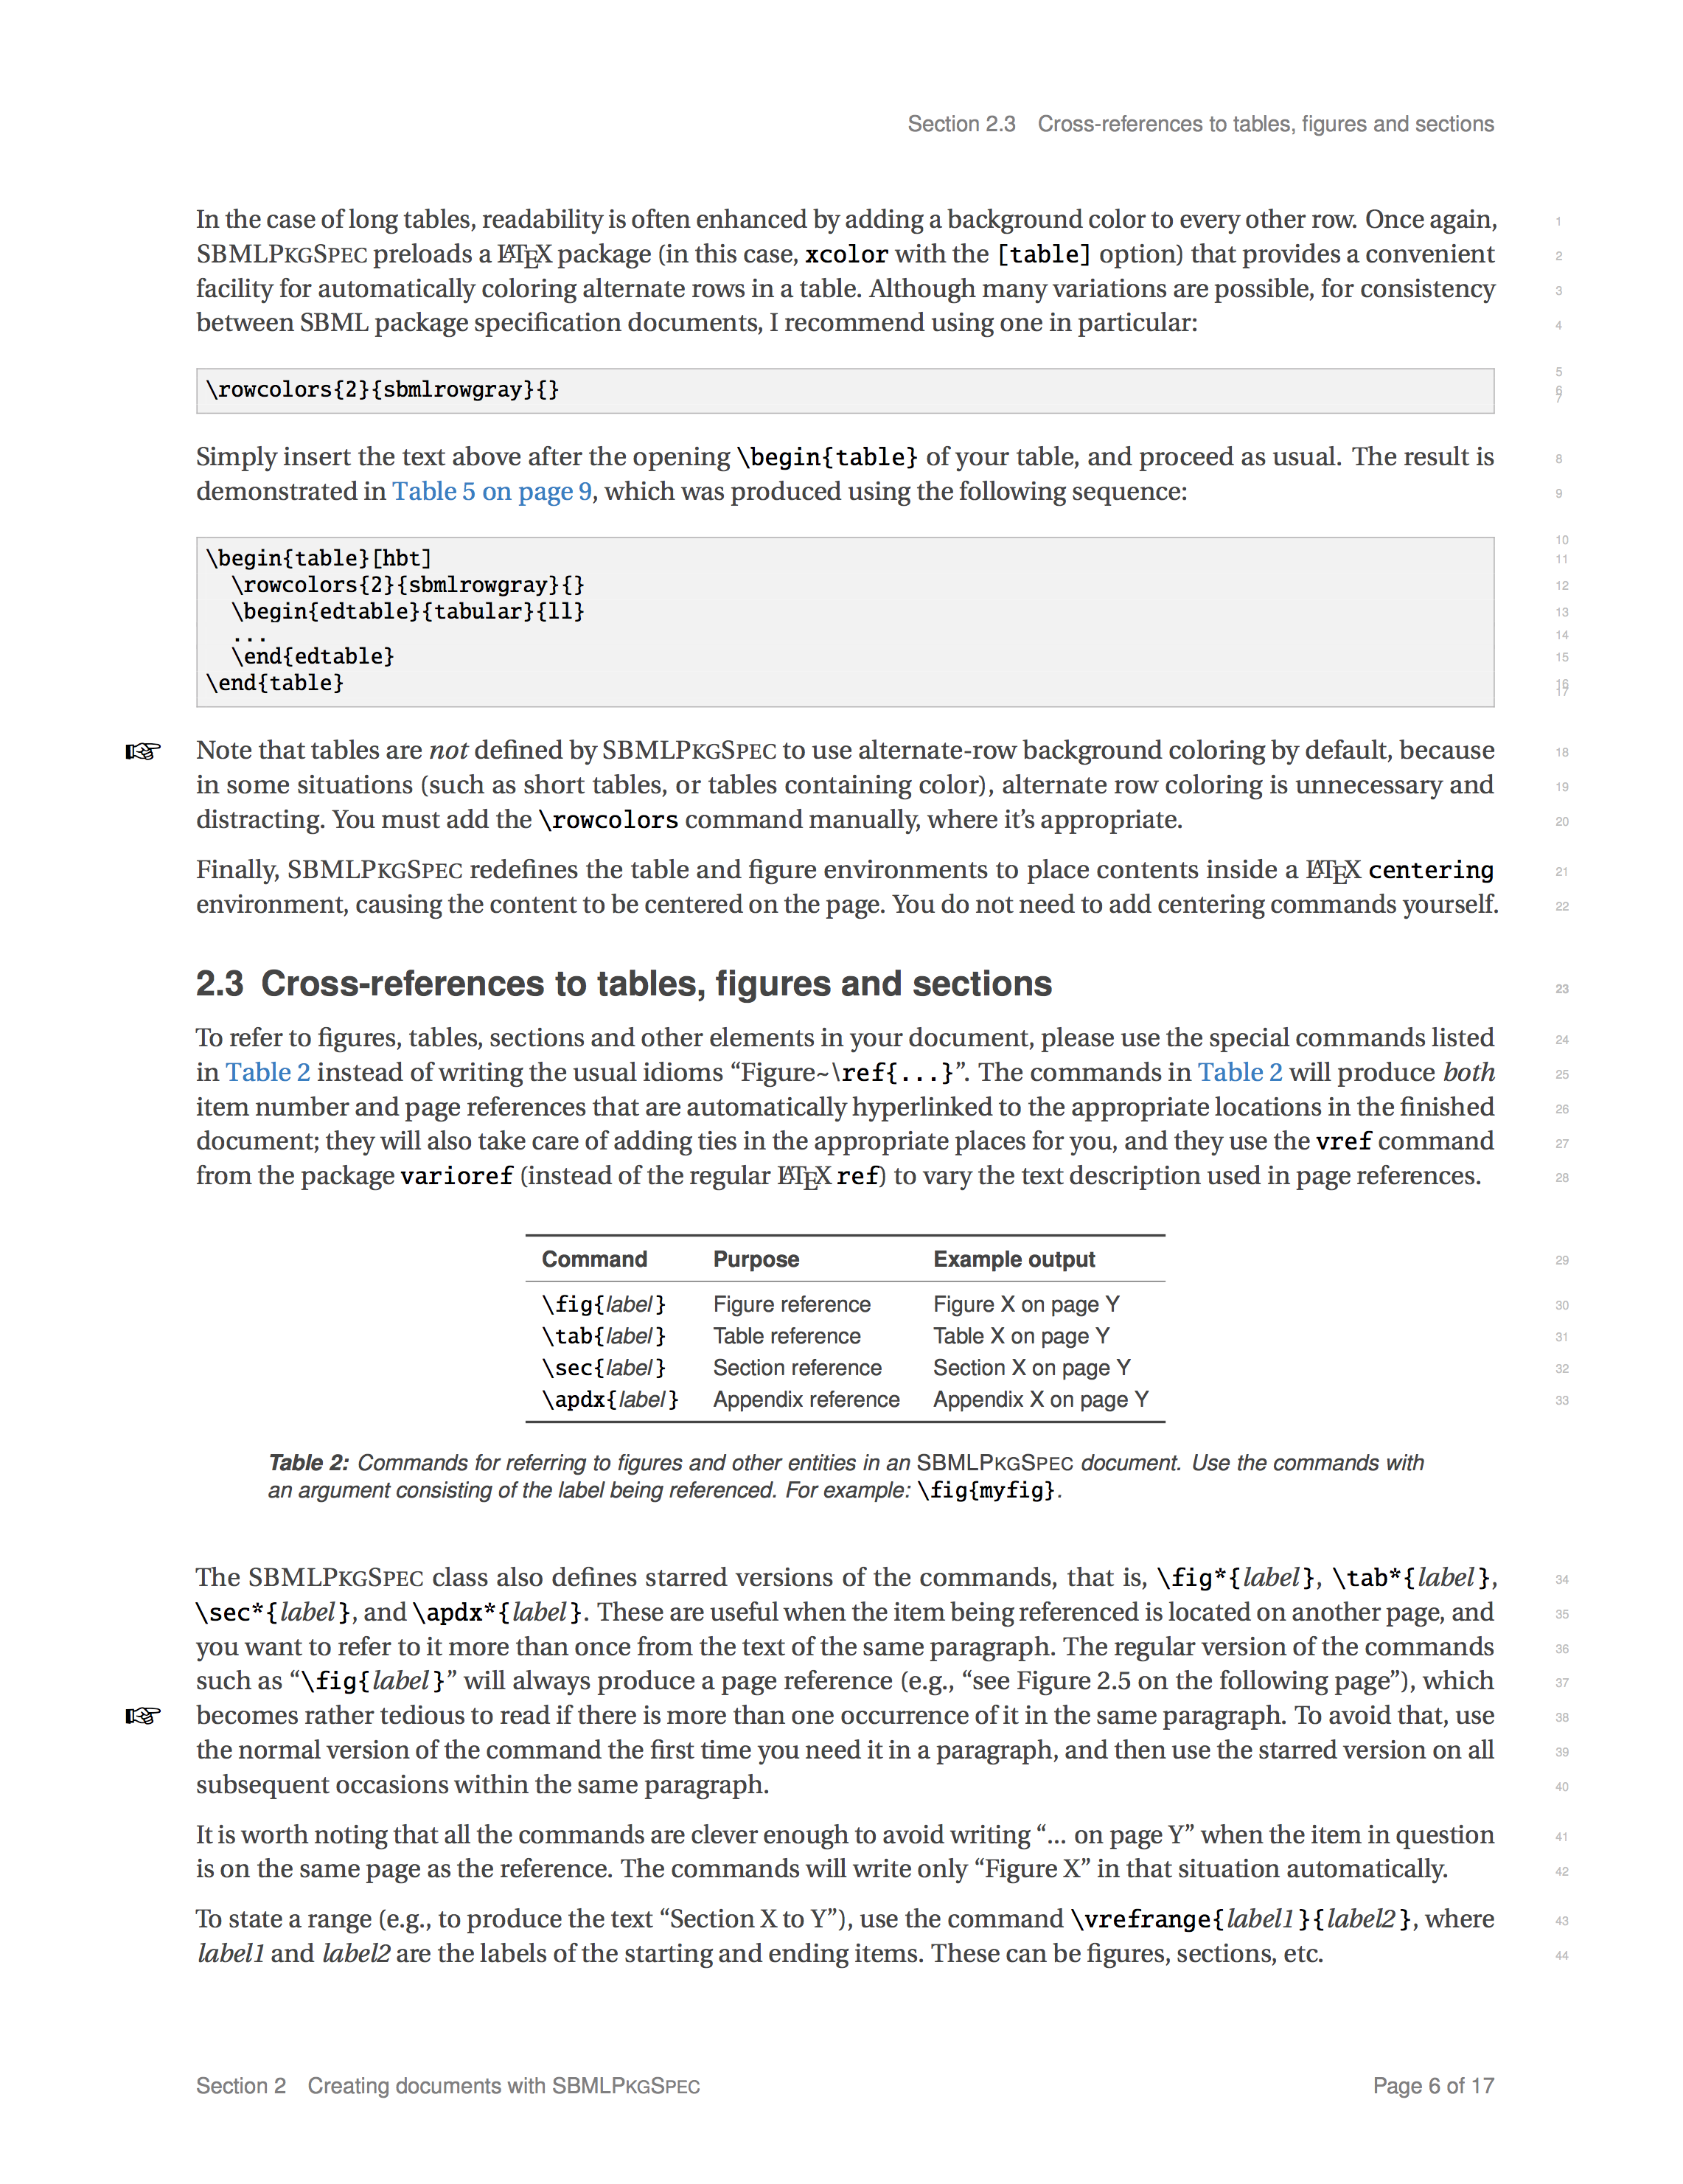
\includegraphics[width=0.9\linewidth]{graphics/sbmlpkgspec-sample-1}}
\caption{A sample page from the \sbmlpkg{} user's guide, illustrating the look and feel of the document and some of its features.}
\end{figure}


%%%%%%%%%%%%%%%%%%%%%%%%%%%%%%%%%%%
%%                               %%
%% Tables                        %%
%%                               %%
%%%%%%%%%%%%%%%%%%%%%%%%%%%%%%%%%%%

%% Use of \listoftables is discouraged.
%%
% \section*{Tables}
% \begin{table}[h!]
% \caption{Sample table title. This is where the description of the table should go.}
%       \begin{tabular}{cccc}
%         \hline
%            & B1  &B2   & B3\\ \hline
%         A1 & 0.1 & 0.2 & 0.3\\
%         A2 & ... & ..  & .\\
%         A3 & ..  & .   & .\\ \hline
%       \end{tabular}
% \end{table}

%%%%%%%%%%%%%%%%%%%%%%%%%%%%%%%%%%%
%%                               %%
%% Additional Files              %%
%%                               %%
%%%%%%%%%%%%%%%%%%%%%%%%%%%%%%%%%%%




\end{document}
